\documentclass[12pt,a4paper]{article}
\usepackage[T1]{fontenc}
\usepackage[utf8]{inputenc}
\usepackage[brazil]{babel}
\usepackage[margin=2.2cm]{geometry}
\usepackage{graphicx}
\usepackage{float}
\usepackage{booktabs}
\usepackage{longtable}
\usepackage{array}
\usepackage{adjustbox}
\usepackage[hidelinks]{hyperref}
\setlength{\parindent}{0pt}
\setlength{\parskip}{0.5em}
\title{Relatorio Geral para Comunicacao}
\author{Analise de Conteudo - Instagram}
\date{Gerado em 2026-04-20 16:42}
\begin{document}
\maketitle
\tableofcontents
\newpage
\section{Leitura rapida para decisao}
\subsection{Escopo da base em linguagem simples}
\begin{itemize}
\item Universo analisado: 27 publicacoes (shortcodes), com 23 delas contendo planilha de comentarios.
\item Volume tratado: 27 posts e 146 comentarios observados.
\item Alcance da comunidade: 129 usuarios distintos comentando no recorte.
\item Sinal de confianca do perfil de commenters: 2.21\% de owners verificados.
\item Leitura pratica: para conversa, o formato lider no recorte foi Video.
\item Regra de leitura: quando aparecer n/d, significa dado nao disponivel na fonte coletada.
\end{itemize}
\subsection{Cinco respostas diretas para comunicacao}
\begin{enumerate}
\item \textbf{Que tipo de conteudo tende a gerar mais conversa?} No recorte atual, Video teve a maior media de comentarios por post (234.77).
\item \textbf{Como aumentar comentarios, e nao apenas likes?} Coautoria mostrou variacao de 3321.60\% em comentarios; CTA ficou em -8.65\%.
\item \textbf{Qual horario priorizar para publicar?} Melhor hora para comentarios: 15h; para visualizacoes: 20h; melhor dia: terca.
\item \textbf{Hashtags ajudam no resultado?} Hashtags variaram 29.75\% em engagement e -16.61\% em comentarios.
\item \textbf{Como elevar a qualidade da conversa?} Coautoria variou o indice de comunidade em n/d; combine coautoria com perguntas objetivas no texto.
\item \textbf{Qual hashtag merece teste prioritario?} No recorte atual, \#caes aparece como referencia de engagement medio entre as hashtags analisadas.
\end{enumerate}
\section{Plano de acao de 30 dias}
\begin{enumerate}
\item Semana 1: priorizar criativos no formato Video para teste de conversa (objetivo: elevar comentarios por post).
\item Semana 2: publicar nos horarios de maior resposta (15h para comentarios e 20h para visualizacoes).
\item Semana 3: executar ao menos 2 testes com coautoria, comparando comentarios e alcance contra a media sem coautoria (referencia de variacao em comentarios: 3321.60\%).
\item Semana 4: revisar hashtags com foco em qualidade e engagement; referencia inicial de engagement no recorte: \#caes.
\item Em todas as semanas: incluir perguntas claras na legenda e acompanhar comentarios qualificados, nao apenas likes.
\end{enumerate}
\section{Metodologia em uma pagina}
\begin{itemize}
\item Fonte dos dados: tabelas de saida do pipeline em analysis\_output/tables e graficos em analysis\_output/charts.
\item Escopo: este documento prioriza decisao de conteudo, horario, coautoria e estrategia de hashtags.
\item Linguagem: termos tecnicos foram traduzidos para facilitar consumo por equipes de comunicacao.
\item Transparencia: quando houver limite de dado, o texto explica impacto pratico na leitura dos resultados.
\end{itemize}
\section{Glossario rapido de metricas}
\subsection{Termos e significados em linguagem simples}
\begin{table}[H]
\centering
\scriptsize
\begin{adjustbox}{max width=\textwidth}
\begin{tabular}{l l}
\toprule
termo & significado simples \\
\midrule
engagement\_rate & Relacao entre interacoes e visualizacoes. Quanto maior, melhor resposta do publico. \\
qualified\_comment\_rate & Percentual de comentarios com mais conteudo util (nao apenas emoji ou palavra curta). \\
discussion\_index & Sinal de conversa ativa, considerando interacao entre pessoas. \\
community\_index & Indicador de criacao de comunidade, com foco em troca recorrente e participacao. \\
lift\_pct & Variacao percentual quando uma estrategia esta presente versus ausente. \\
n/d & Dado nao disponivel na fonte coletada. \\
\bottomrule
\end{tabular}
\end{adjustbox}
\caption{Termos e significados em linguagem simples}
\label{tab:glossario}
\end{table}

\section{Tabelas essenciais para tomada de decisao}
\subsection{KPI geral}
\begin{table}[H]
\centering
\scriptsize
\begin{adjustbox}{max width=\textwidth}
\begin{tabular}{l r}
\toprule
indicador & valor \\
\midrule
total\_shortcodes & 27 \\
shortcodes\_com\_comments & 23 \\
shortcodes\_sem\_comments & 4 \\
posts\_processados & 27 \\
comentarios\_observados & 146 \\
usuarios\_unicos\_comentando & 129 \\
percentual\_owners\_verificados & 2.21\% \\
\bottomrule
\end{tabular}
\end{adjustbox}
\caption{KPI geral}
\label{tab:kpi}
\end{table}

\subsection{Comparacao por tipo de conteudo (foco em conversa)}
\begin{table}[H]
\centering
\scriptsize
\begin{adjustbox}{max width=\textwidth}
\begin{tabular}{l r r l r r}
\toprule
tipo & posts & num comentarios & engagement rate & qualified comment rate & community index \\
\midrule
Video & 13 & 234.77 & 21.7877 & 0.2607 & 0.1030 \\
Sidecar & 8 & 127.38 & n/d & 0.4563 & 0.1230 \\
Image & 6 & 36 & n/d & 0.3500 & 0.0833 \\
\bottomrule
\end{tabular}
\end{adjustbox}
\caption{Comparacao por tipo de conteudo (foco em conversa)}
\label{tab:tipo}
\end{table}

\subsection{Melhor horario por resultado medio}
\begin{table}[H]
\centering
\scriptsize
\begin{adjustbox}{max width=\textwidth}
\begin{tabular}{r r r r r}
\toprule
post hour & posts & avg comments & avg views & avg engagement rate \\
\midrule
9 & 1 & 163 & n/d & n/d \\
10 & 2 & 0.50 & 87 & 1.4828 \\
11 & 5 & 8.60 & 109 & 20.2028 \\
12 & 4 & 66 & 437.50 & 16.3435 \\
14 & 1 & 0 & n/d & n/d \\
15 & 2 & 467 & n/d & n/d \\
16 & 3 & 40.33 & n/d & n/d \\
17 & 4 & 307.25 & 515.75 & 18.6456 \\
18 & 3 & 231 & 613 & 30.3516 \\
20 & 2 & 419.50 & 1025 & 43.0273 \\
\bottomrule
\end{tabular}
\end{adjustbox}
\caption{Melhor horario por resultado medio}
\label{tab:hora}
\end{table}

\subsection{Melhor dia da semana por resultado medio}
\begin{table}[H]
\centering
\scriptsize
\begin{adjustbox}{max width=\textwidth}
\begin{tabular}{l r r r r}
\toprule
post weekday & posts & avg comments & avg views & avg engagement rate \\
\midrule
segunda & 7 & 121.43 & 309.75 & 16.0312 \\
terca & 6 & 302 & 828 & 46.1967 \\
quarta & 5 & 89.20 & 753.50 & 18.4844 \\
quinta & 7 & 102.57 & 248.50 & 13.4766 \\
sexta & 2 & 230.50 & 711 & 35.8467 \\
\bottomrule
\end{tabular}
\end{adjustbox}
\caption{Melhor dia da semana por resultado medio}
\label{tab:dia}
\end{table}

\subsection{Hashtags com maior relevancia no recorte}
\begin{table}[H]
\centering
\scriptsize
\begin{adjustbox}{max width=\textwidth}
\begin{tabular}{l r r l r}
\toprule
hashtag & posts & avg comments & avg engagement rate & avg qualified comment rate \\
\midrule
\#ufsm & 16 & 150.44 & 23.8947 & 0.3327 \\
\#silveira & 5 & 467.40 & 32.9917 & 0.3483 \\
\#ufsmdaquiparaomundo & 4 & 507.50 & 39.3551 & 0.3229 \\
\#souufsm & 4 & 5 & 1.1559 & 0.3264 \\
\#extensaouniversitaria & 3 & 2.67 & n/d & 0.2500 \\
\#silveiraufsm & 2 & 599.50 & 37.5190 & 0.2292 \\
\#cinema & 1 & 1 & 0.0000 & 0.0000 \\
\#conexoesquetransformam & 1 & 8 & n/d & 0.2500 \\
\#conscienciaafricana & 1 & 13 & 18.7857 & 0.1111 \\
\#abelhas & 1 & 9 & n/d & 0.2222 \\
\#agendacultural & 1 & 4 & n/d & 0.7500 \\
\#antigareitoria & 1 & 0 & n/d & n/d \\
\bottomrule
\end{tabular}
\end{adjustbox}
\caption{Hashtags com maior relevancia no recorte}
\label{tab:hashtags}
\end{table}

\subsection{Efeito das principais estrategias (coautoria, CTA e hashtags)}
\begin{table}[H]
\centering
\scriptsize
\begin{adjustbox}{max width=\textwidth}
\begin{tabular}{l l r r r r r}
\toprule
feature & metric & with feature & without feature & lift pct & n with & n without \\
\midrule
has\_coauthors & num\_comentarios & 171.08 & 5 & 3321.60\% & 25 & 2 \\
has\_hashtags & visualizacoes & 619.88 & 229.60 & 169.98\% & 18 & 9 \\
has\_cta & community\_index & 0.03 & 0.12 & -77.25\% & 5 & 22 \\
has\_hashtags & community\_index & 0.08 & 0.16 & -51.88\% & 18 & 9 \\
has\_hashtags & engagement\_rate & 23.89 & 18.42 & 29.75\% & 18 & 9 \\
has\_hashtags & num\_comentarios & 148.89 & 178.56 & -16.61\% & 18 & 9 \\
has\_cta & num\_comentarios & 147.40 & 161.36 & -8.65\% & 5 & 22 \\
has\_hashtags & new\_commenter\_share & 0.97 & 0.90 & 8.40\% & 18 & 9 \\
has\_cta & new\_commenter\_share & 1 & 0.93 & 7.14\% & 5 & 22 \\
has\_coauthors & new\_commenter\_share & 0.94 & 1 & -6.03\% & 25 & 2 \\
has\_coauthors & visualizacoes & 469.77 & n/d & n/d & 25 & 2 \\
has\_coauthors & engagement\_rate & 21.79 & n/d & n/d & 25 & 2 \\
has\_coauthors & community\_index & 0.12 & 0 & n/d & 25 & 2 \\
has\_cta & visualizacoes & n/d & 469.77 & n/d & 5 & 22 \\
has\_cta & engagement\_rate & n/d & 21.79 & n/d & 5 & 22 \\
\bottomrule
\end{tabular}
\end{adjustbox}
\caption{Efeito das principais estrategias (coautoria, CTA e hashtags)}
\label{tab:features}
\end{table}

\subsection{Coautores com maior participacao no recorte}
\begin{table}[H]
\centering
\scriptsize
\begin{adjustbox}{max width=\textwidth}
\begin{tabular}{l r r r r r}
\toprule
coautor & posts & avg comments & avg views & avg engagement rate & avg qualified comment rate \\
\midrule
ufsm.br & 18 & 87.33 & 225.50 & 16.5175 & 0.2312 \\
silveirapodrao & 10 & 414.50 & 958.50 & 36.9674 & 0.3097 \\
zeloufsm & 8 & 464.62 & 958.50 & 36.9674 & 0.3247 \\
extensaoufsm & 5 & 216 & 458.33 & 31.7607 & 0.2257 \\
radiosufsm & 4 & 66.25 & 437.50 & 16.3435 & 0.5153 \\
ufsmpm & 2 & 4.50 & 14 & 0.4286 & 0.5714 \\
citurdes & 1 & 4 & 9 & 0.3333 & 0.2500 \\
centrodeconvencoes.ufsm & 1 & 0 & 87 & 1.4828 & n/d \\
dce.ufsm & 1 & 8 & n/d & n/d & 0.2500 \\
dag\_ufsm & 1 & 1 & 14 & 0.0000 & 0.0000 \\
gabinetereitoriaufsm & 1 & 767 & 1329 & 38.4026 & 0.1250 \\
fazendoarteufsm & 1 & 4 & n/d & n/d & 0.7500 \\
\bottomrule
\end{tabular}
\end{adjustbox}
\caption{Coautores com maior participacao no recorte}
\label{tab:coautores}
\end{table}

\subsection{Usuarios mais recorrentes em comentarios}
\begin{table}[H]
\centering
\scriptsize
\begin{adjustbox}{max width=\textwidth}
\begin{tabular}{l r r r r}
\toprule
owner username norm & comentarios & posts distintos & comentarios qualificados & taxa perguntas \\
\midrule
dupladedoismartinmabel & 4 & 1 & 0 & 0 \\
ufsmpm & 4 & 1 & 0 & 0 \\
djarts\_8 & 3 & 2 & 0 & 0 \\
albummbel & 2 & 2 & 0 & 0 \\
ateliefogo & 2 & 2 & 0 & 0 \\
elisangelapessoa46 & 2 & 2 & 2 & 0 \\
geanefedrigo & 2 & 2 & 0 & 0 \\
gislaine7166 & 2 & 2 & 0 & 0 \\
radiosufsm & 2 & 2 & 2 & 0 \\
claudia\_m\_ferrari & 2 & 1 & 1 & 0.50 \\
nelci.lourenco.1612 & 2 & 1 & 0 & 0 \\
robertakt & 2 & 1 & 1 & 0.50 \\
\_.jeds & 1 & 1 & 0 & 0 \\
\_otiiago\_ & 1 & 1 & 0 & 0 \\
a\_myreya\_ & 1 & 1 & 0 & 0 \\
\bottomrule
\end{tabular}
\end{adjustbox}
\caption{Usuarios mais recorrentes em comentarios}
\label{tab:commenters}
\end{table}

\subsection{Guia rapido de leitura para reuniao}
\begin{table}[H]
\centering
\scriptsize
\begin{adjustbox}{max width=\textwidth}
\begin{tabular}{l l l}
\toprule
pergunta & acao recomendada & indicador chave \\
\midrule
Formato de conteudo & Priorizar formatos que lideram em comentarios e validar consistencia semanal. & num\_comentarios \\
Horario de publicacao & Concentrar publicacoes nas janelas de melhor resposta e comparar com horario controle. & avg\_comments por hora \\
Uso de coautoria & Usar coautoria quando objetivo for ampliar conversa e alcance. & lift\_pct em comentarios e visualizacoes \\
Qualidade da conversa & Acompanhar comentarios qualificados e taxa de perguntas em paralelo com volume. & qualified\_comment\_rate \\
\bottomrule
\end{tabular}
\end{adjustbox}
\caption{Guia rapido de leitura para reuniao}
\label{tab:guia\_reuniao}
\end{table}

\section{Figuras comentadas}
\begin{figure}[H]
\centering
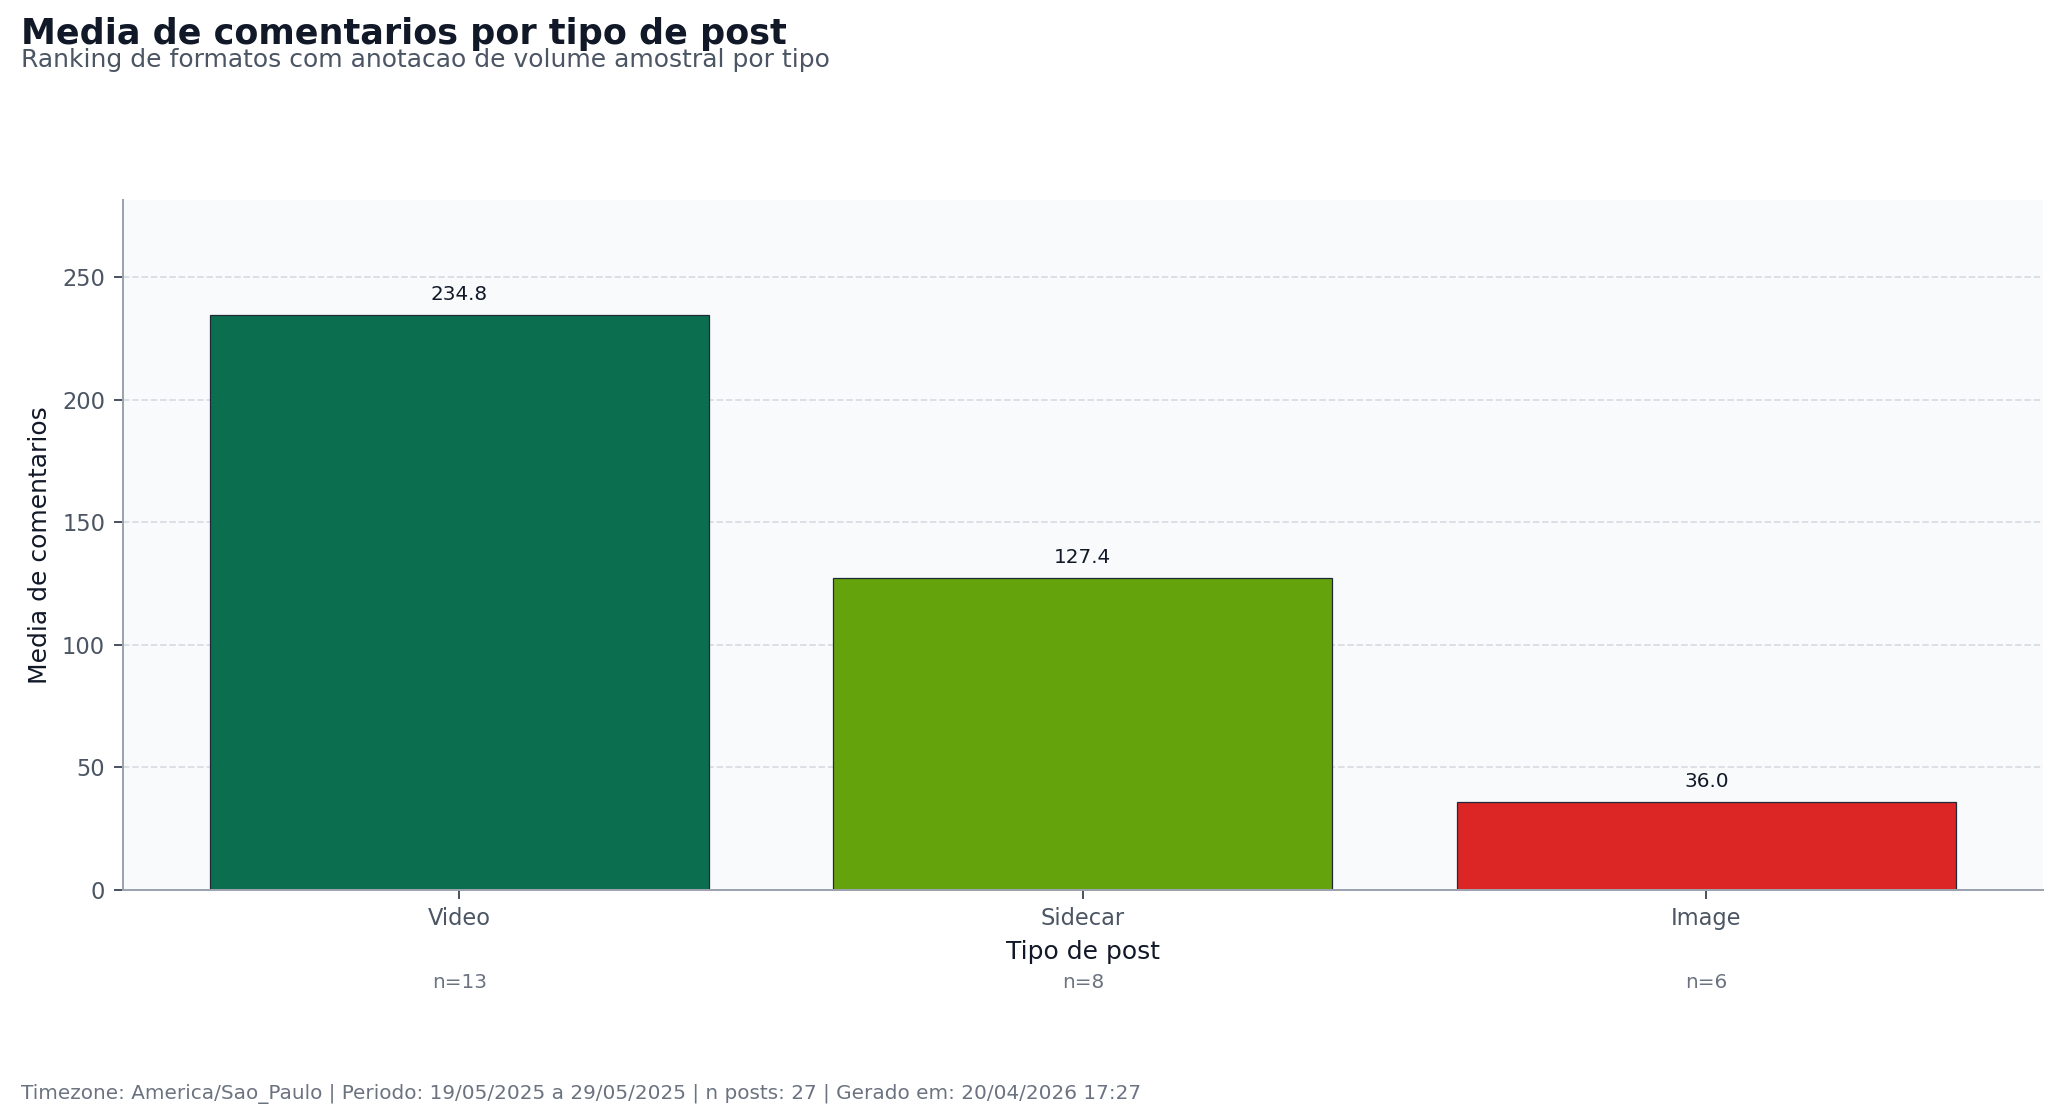
\includegraphics[width=0.93\textwidth]{charts/post_type_avg_comments.png}
\caption{Figura 1: Media de comentarios por tipo de post}
\end{figure}
\textit{Leitura rapida: Mostra quais formatos puxam mais conversa por post.}

\begin{figure}[H]
\centering
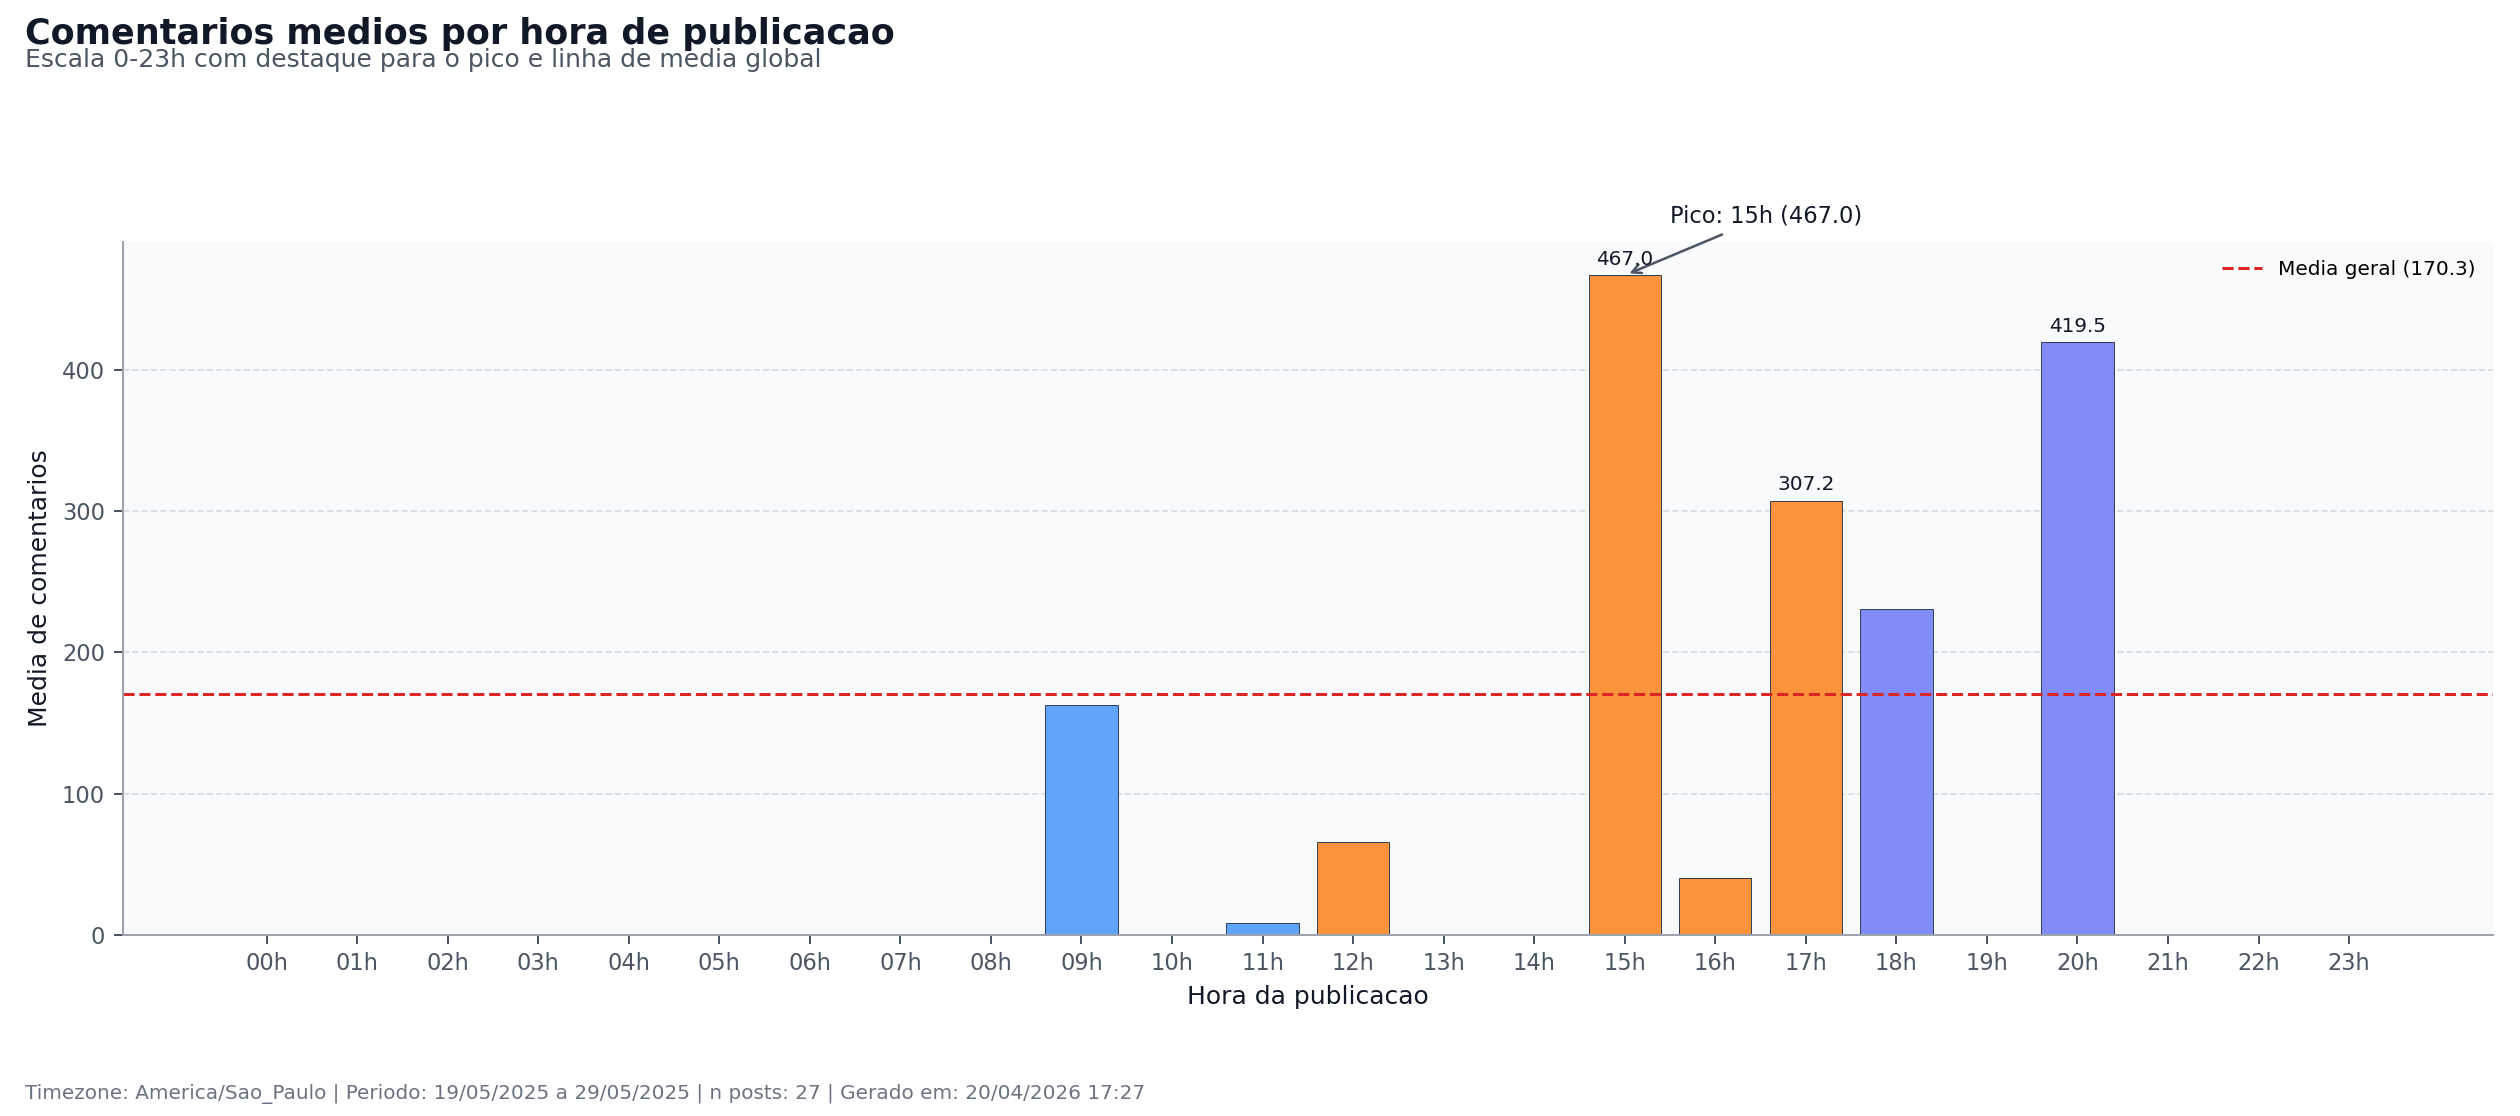
\includegraphics[width=0.93\textwidth]{charts/timing_hour_avg_comments.png}
\caption{Figura 2: Comentarios medios por hora de publicacao}
\end{figure}
\textit{Leitura rapida: Ajuda a escolher a melhor janela de horario para publicar.}

\begin{figure}[H]
\centering
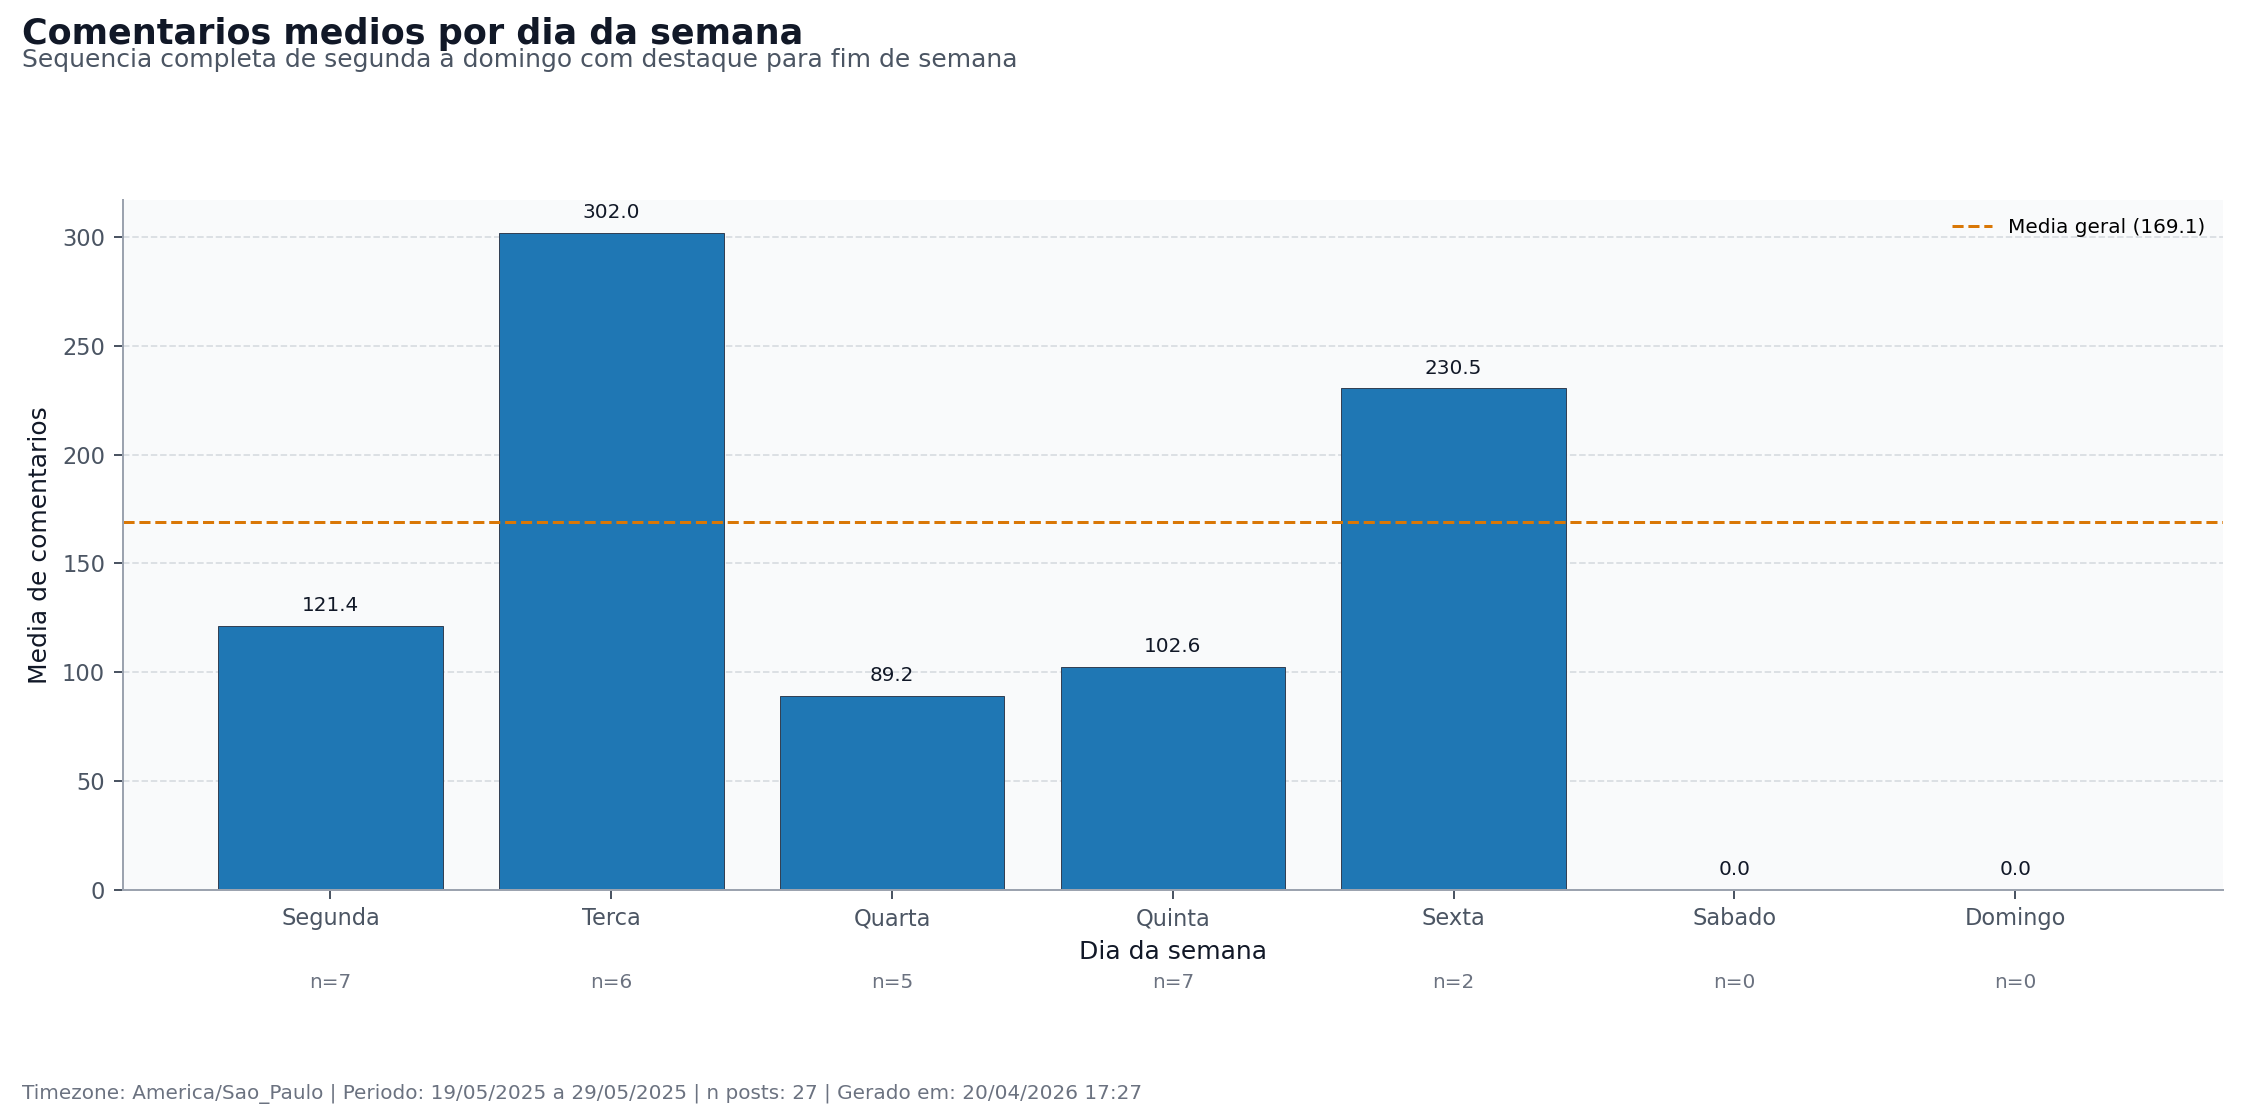
\includegraphics[width=0.93\textwidth]{charts/timing_weekday_avg_comments.png}
\caption{Figura 3: Comentarios medios por dia da semana}
\end{figure}
\textit{Leitura rapida: Indica os dias com maior chance de receber comentarios.}

\begin{figure}[H]
\centering
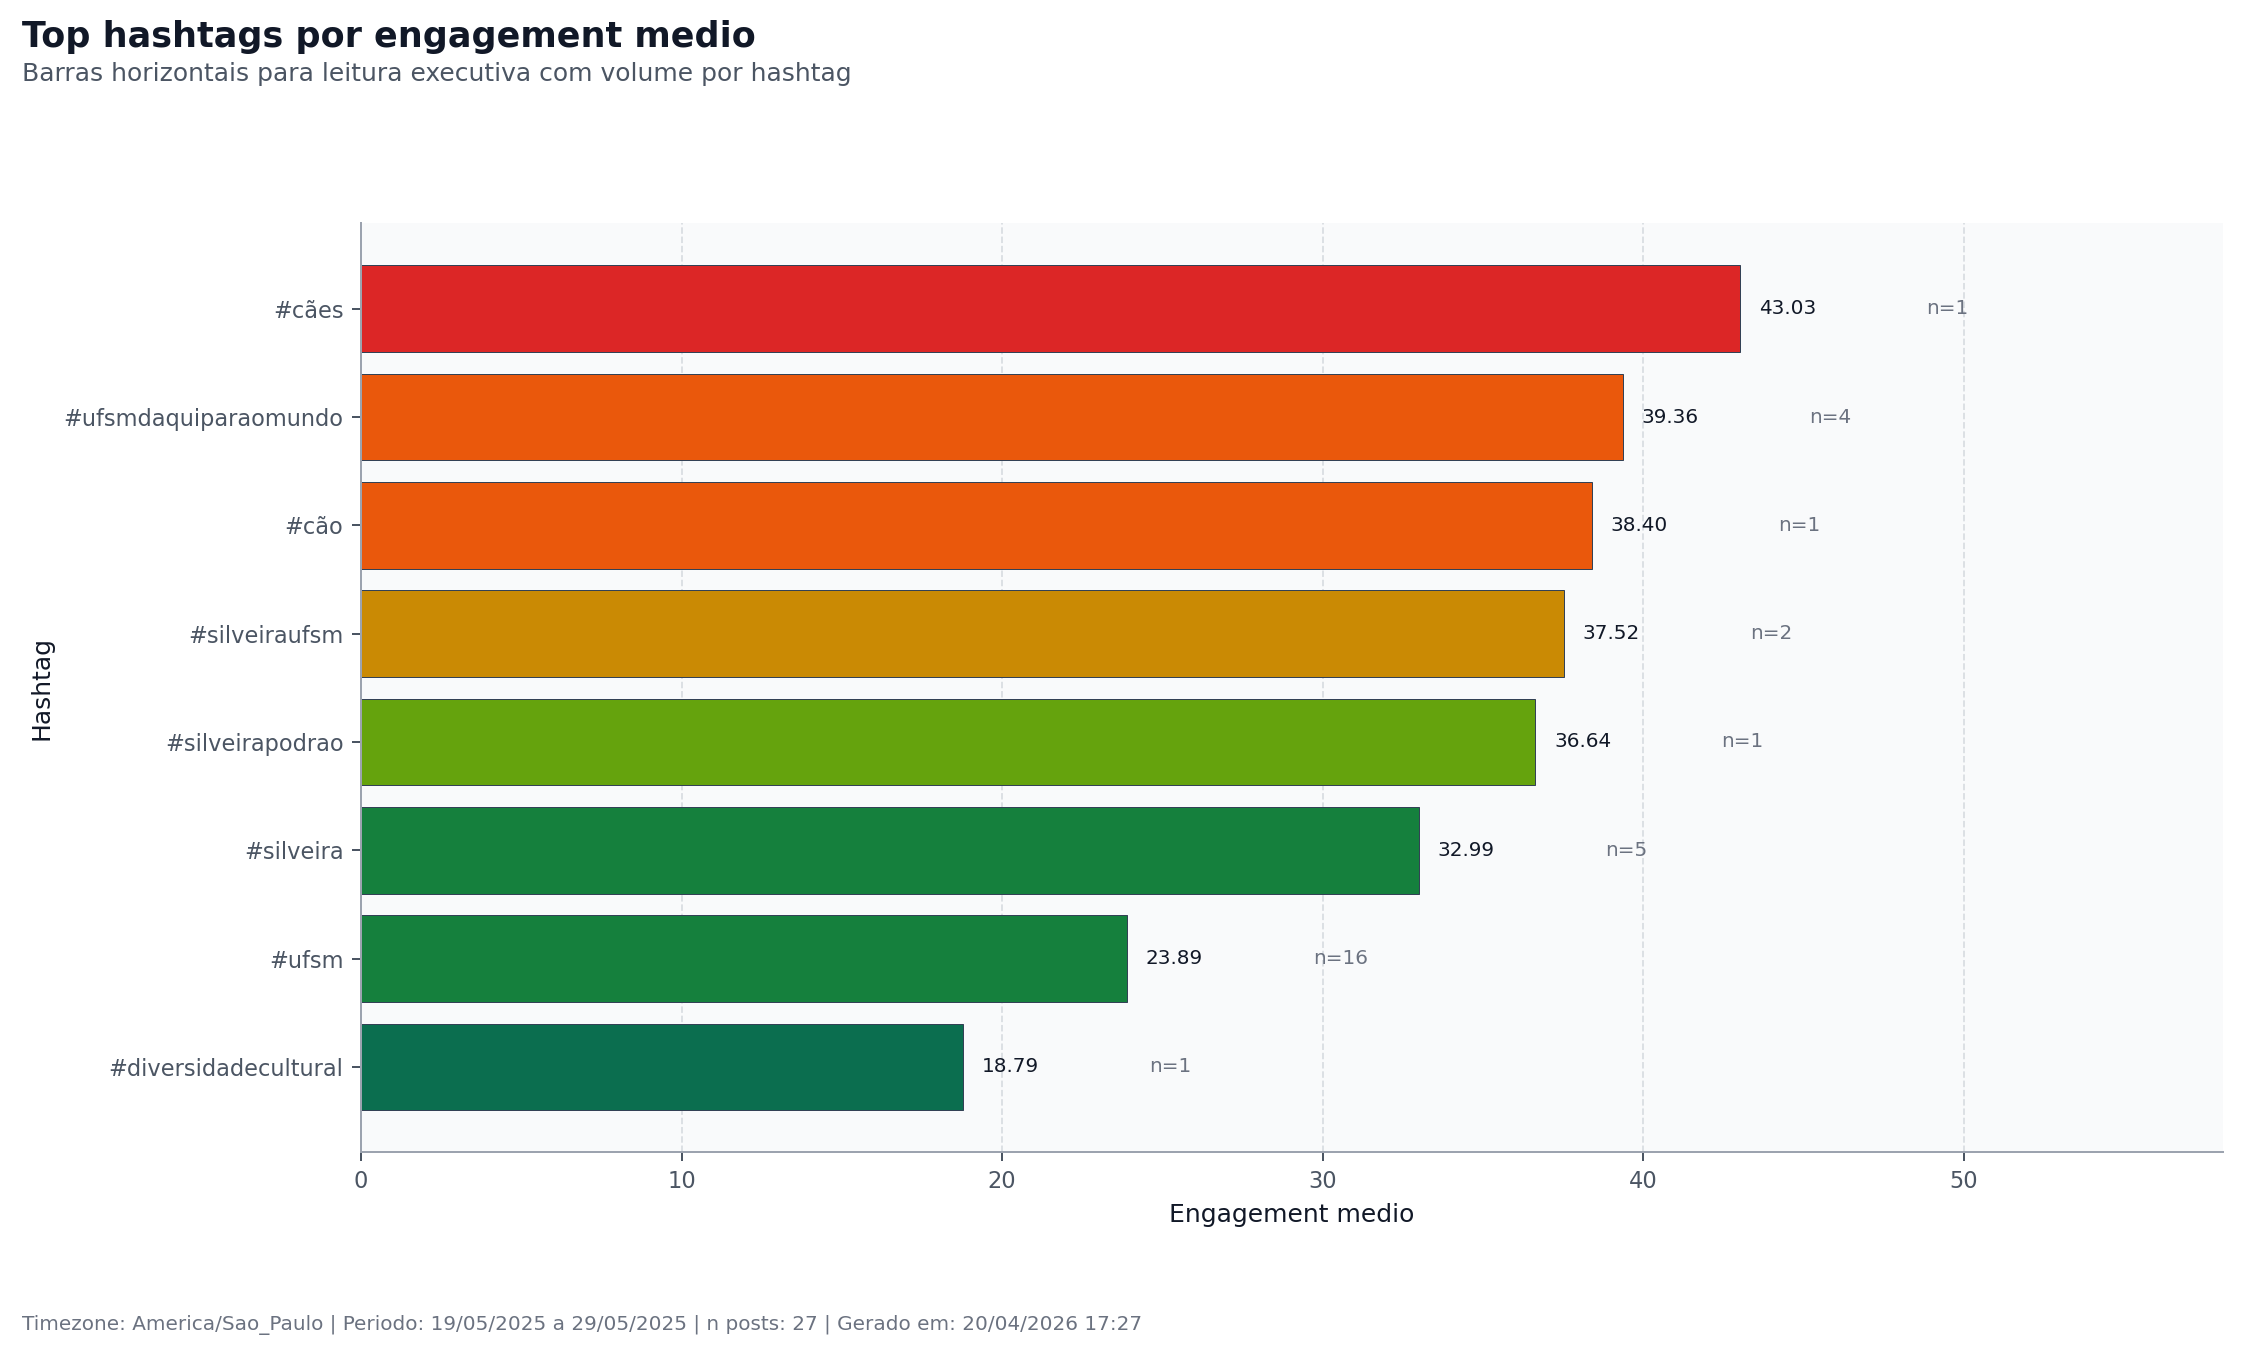
\includegraphics[width=0.93\textwidth]{charts/top_hashtags_engagement.png}
\caption{Figura 4: Top hashtags por engagement medio}
\end{figure}
\textit{Leitura rapida: Resume hashtags com melhor equilibrio entre alcance e interacao.}

\begin{figure}[H]
\centering
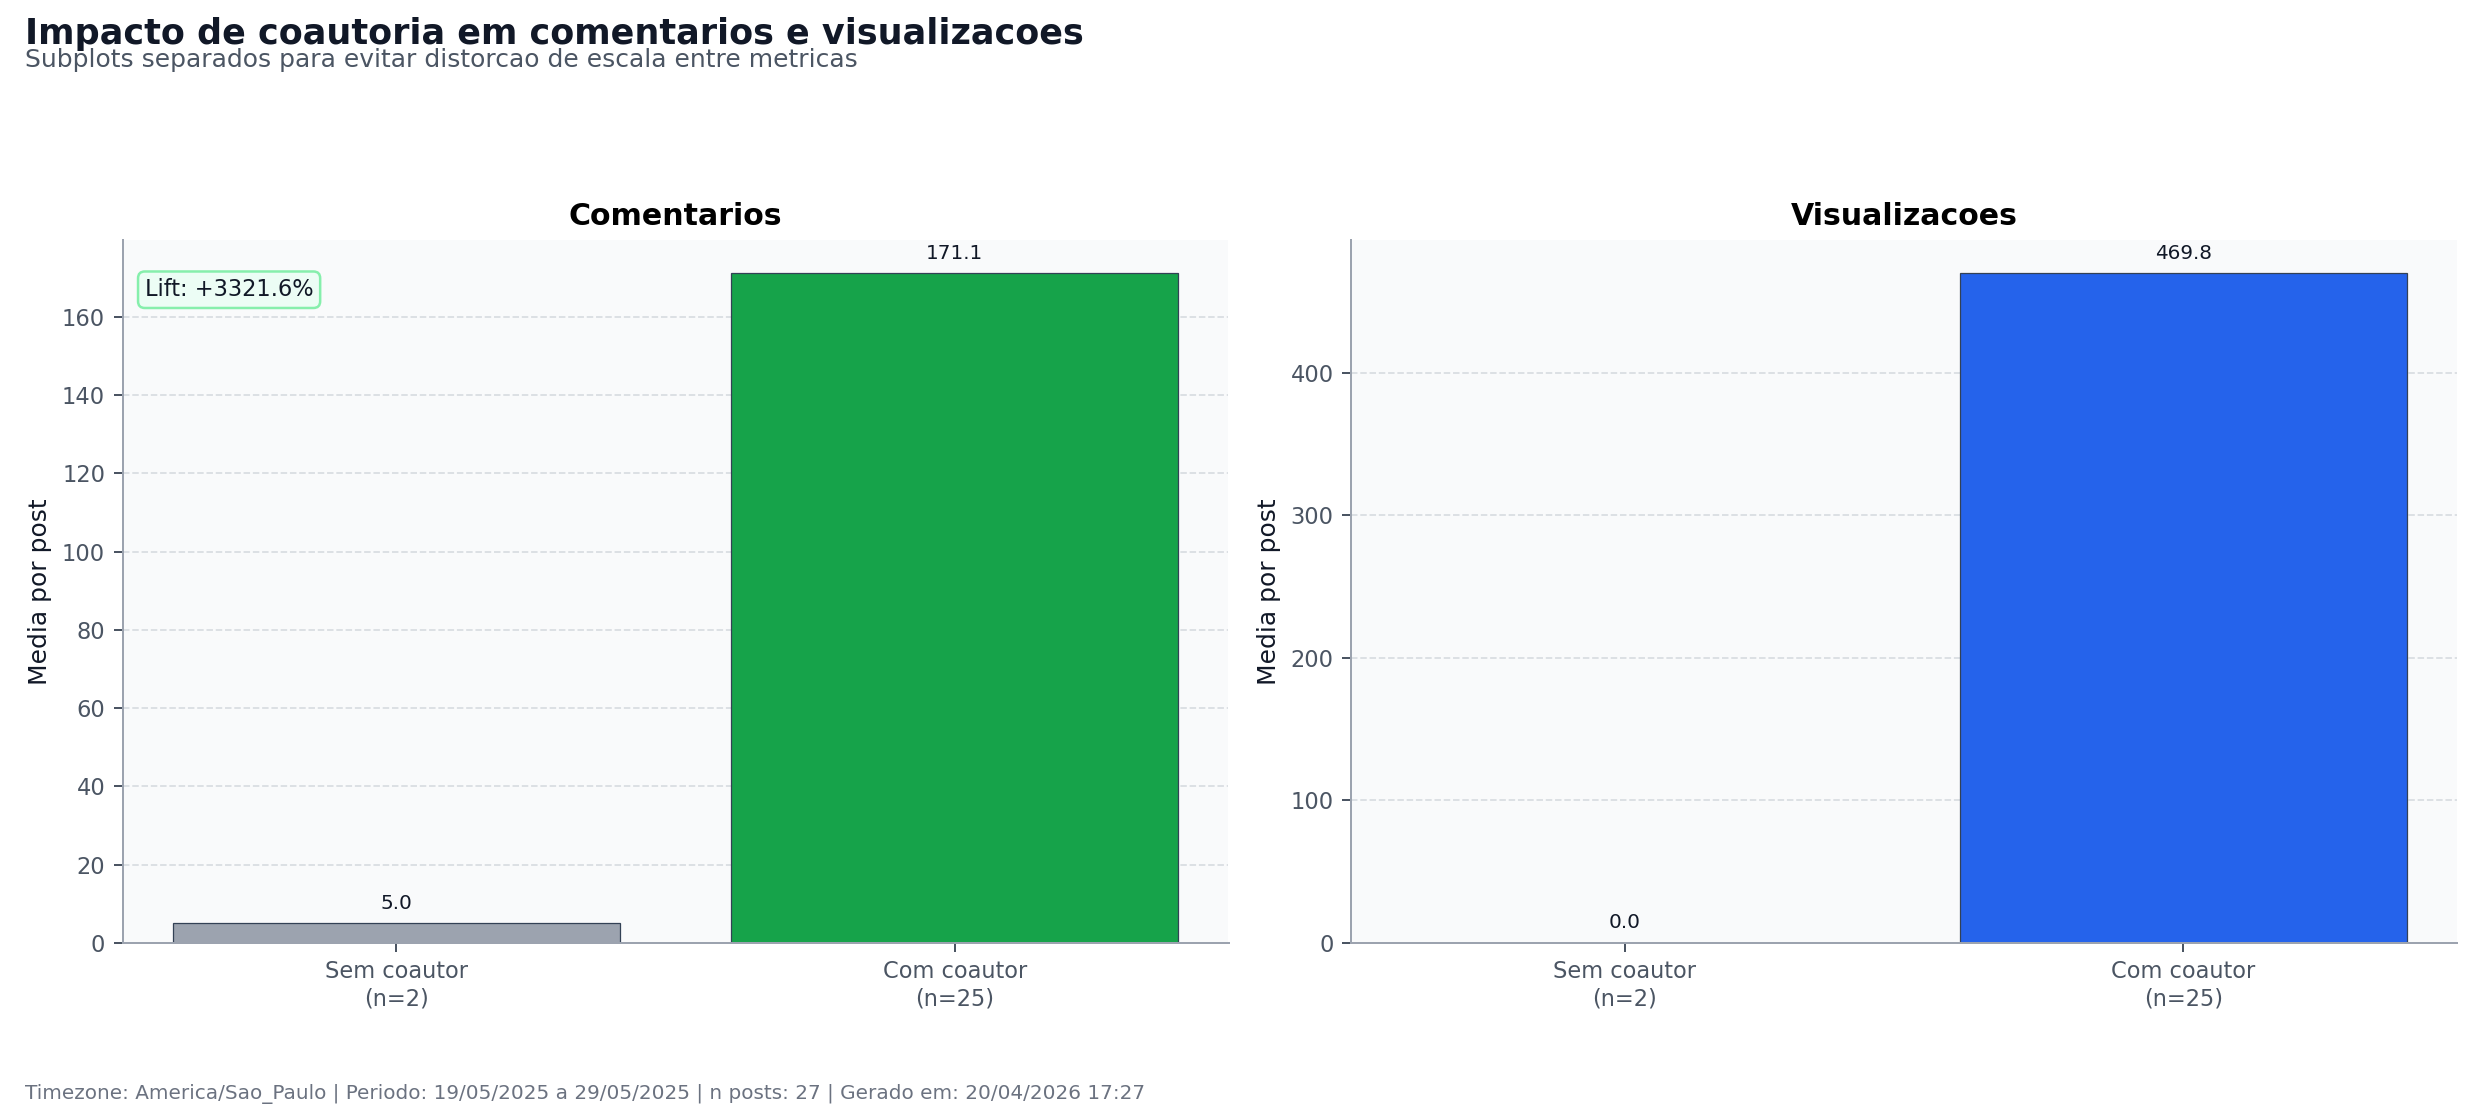
\includegraphics[width=0.93\textwidth]{charts/coauthor_impact_comments_views.png}
\caption{Figura 5: Impacto de coautoria em comentarios e visualizacoes}
\end{figure}
\textit{Leitura rapida: Compara resultado medio de posts com e sem coautoria.}

\begin{figure}[H]
\centering
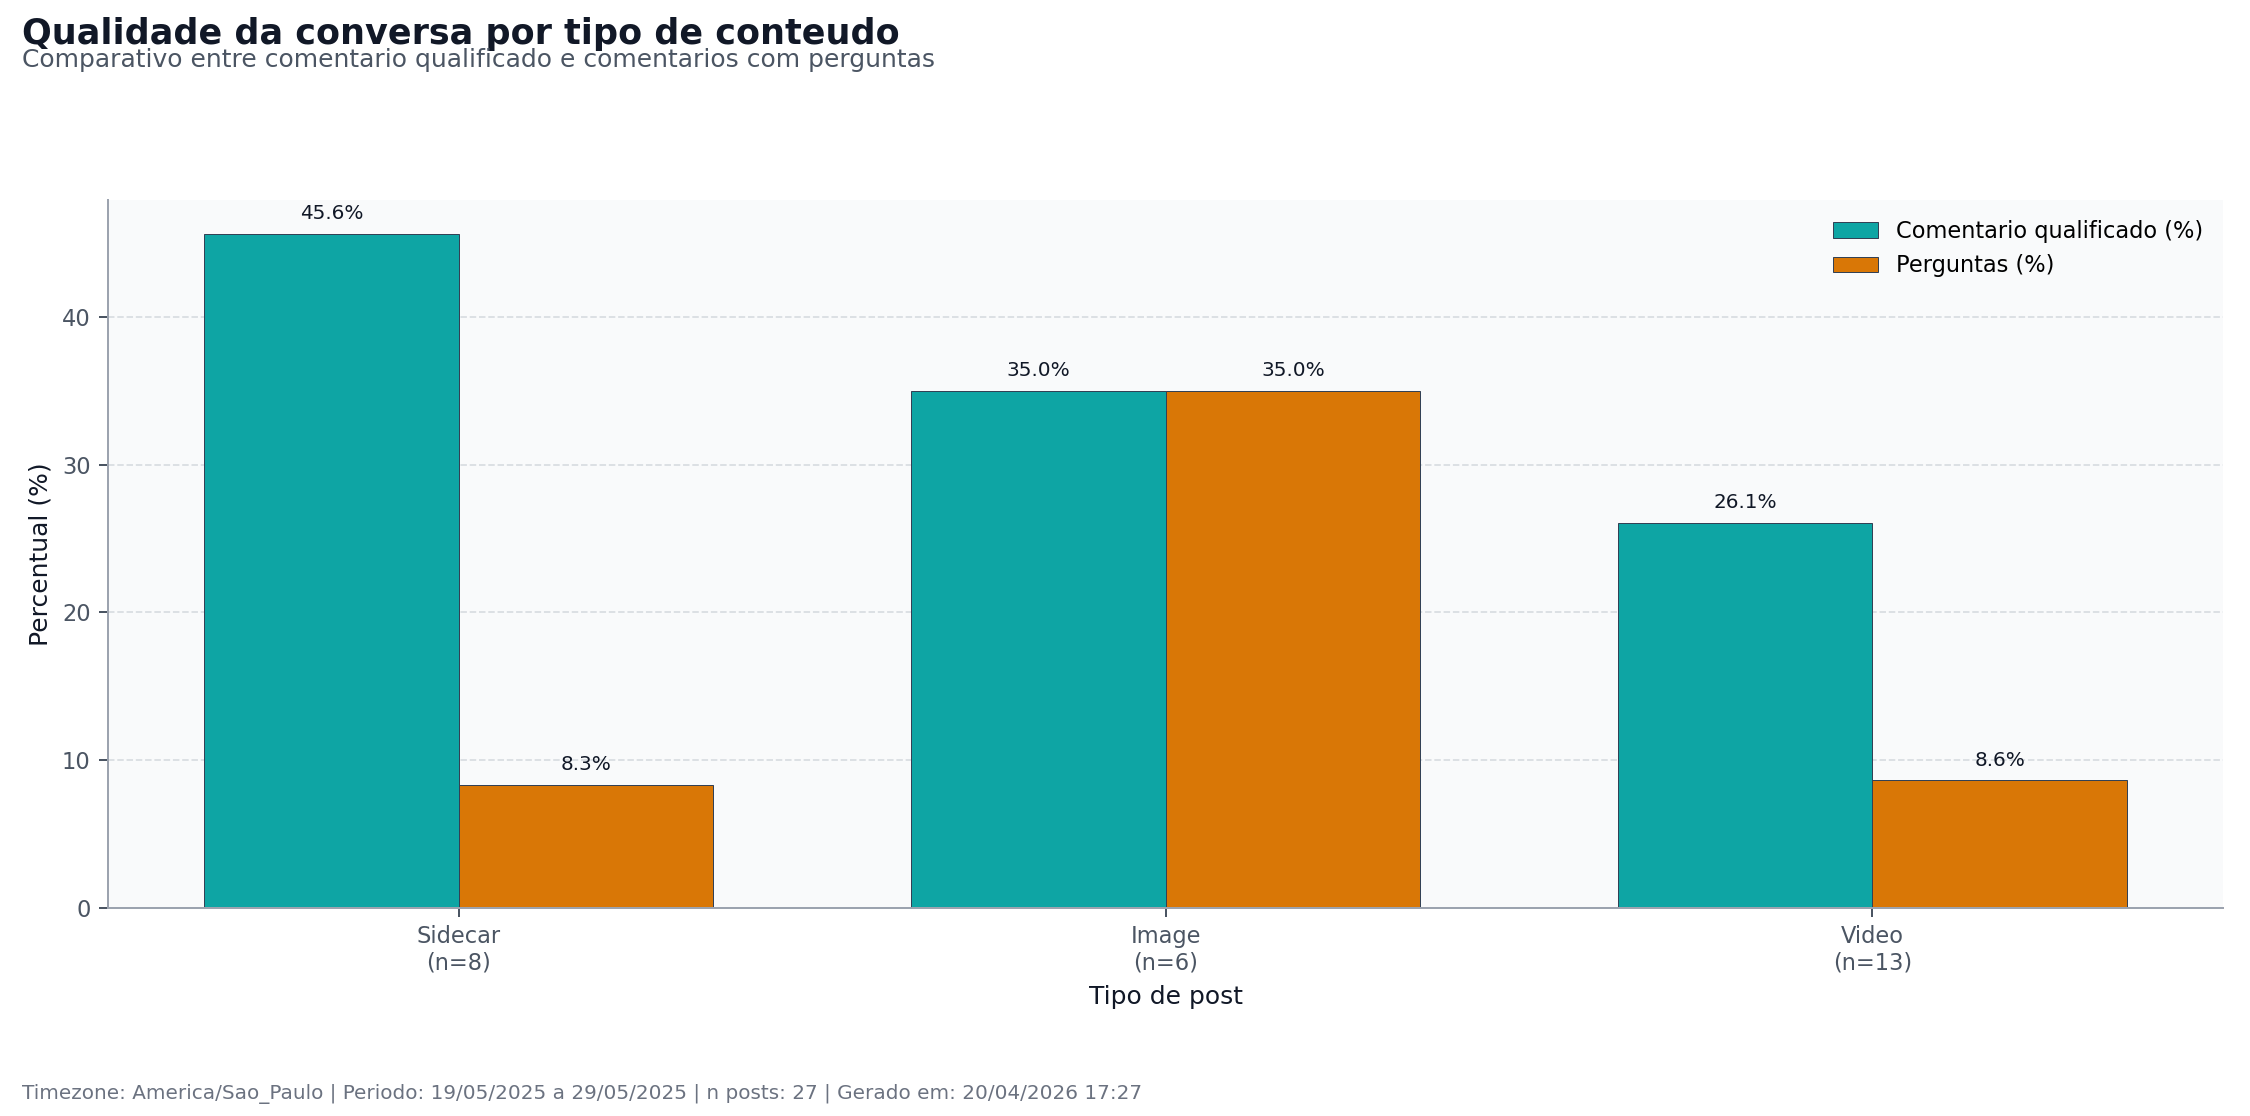
\includegraphics[width=0.93\textwidth]{charts/quality_by_type.png}
\caption{Figura 6: Qualidade da conversa por tipo de conteudo}
\end{figure}
\textit{Leitura rapida: Mostra se o tipo de conteudo gera comentario mais qualificado.}

\begin{figure}[H]
\centering
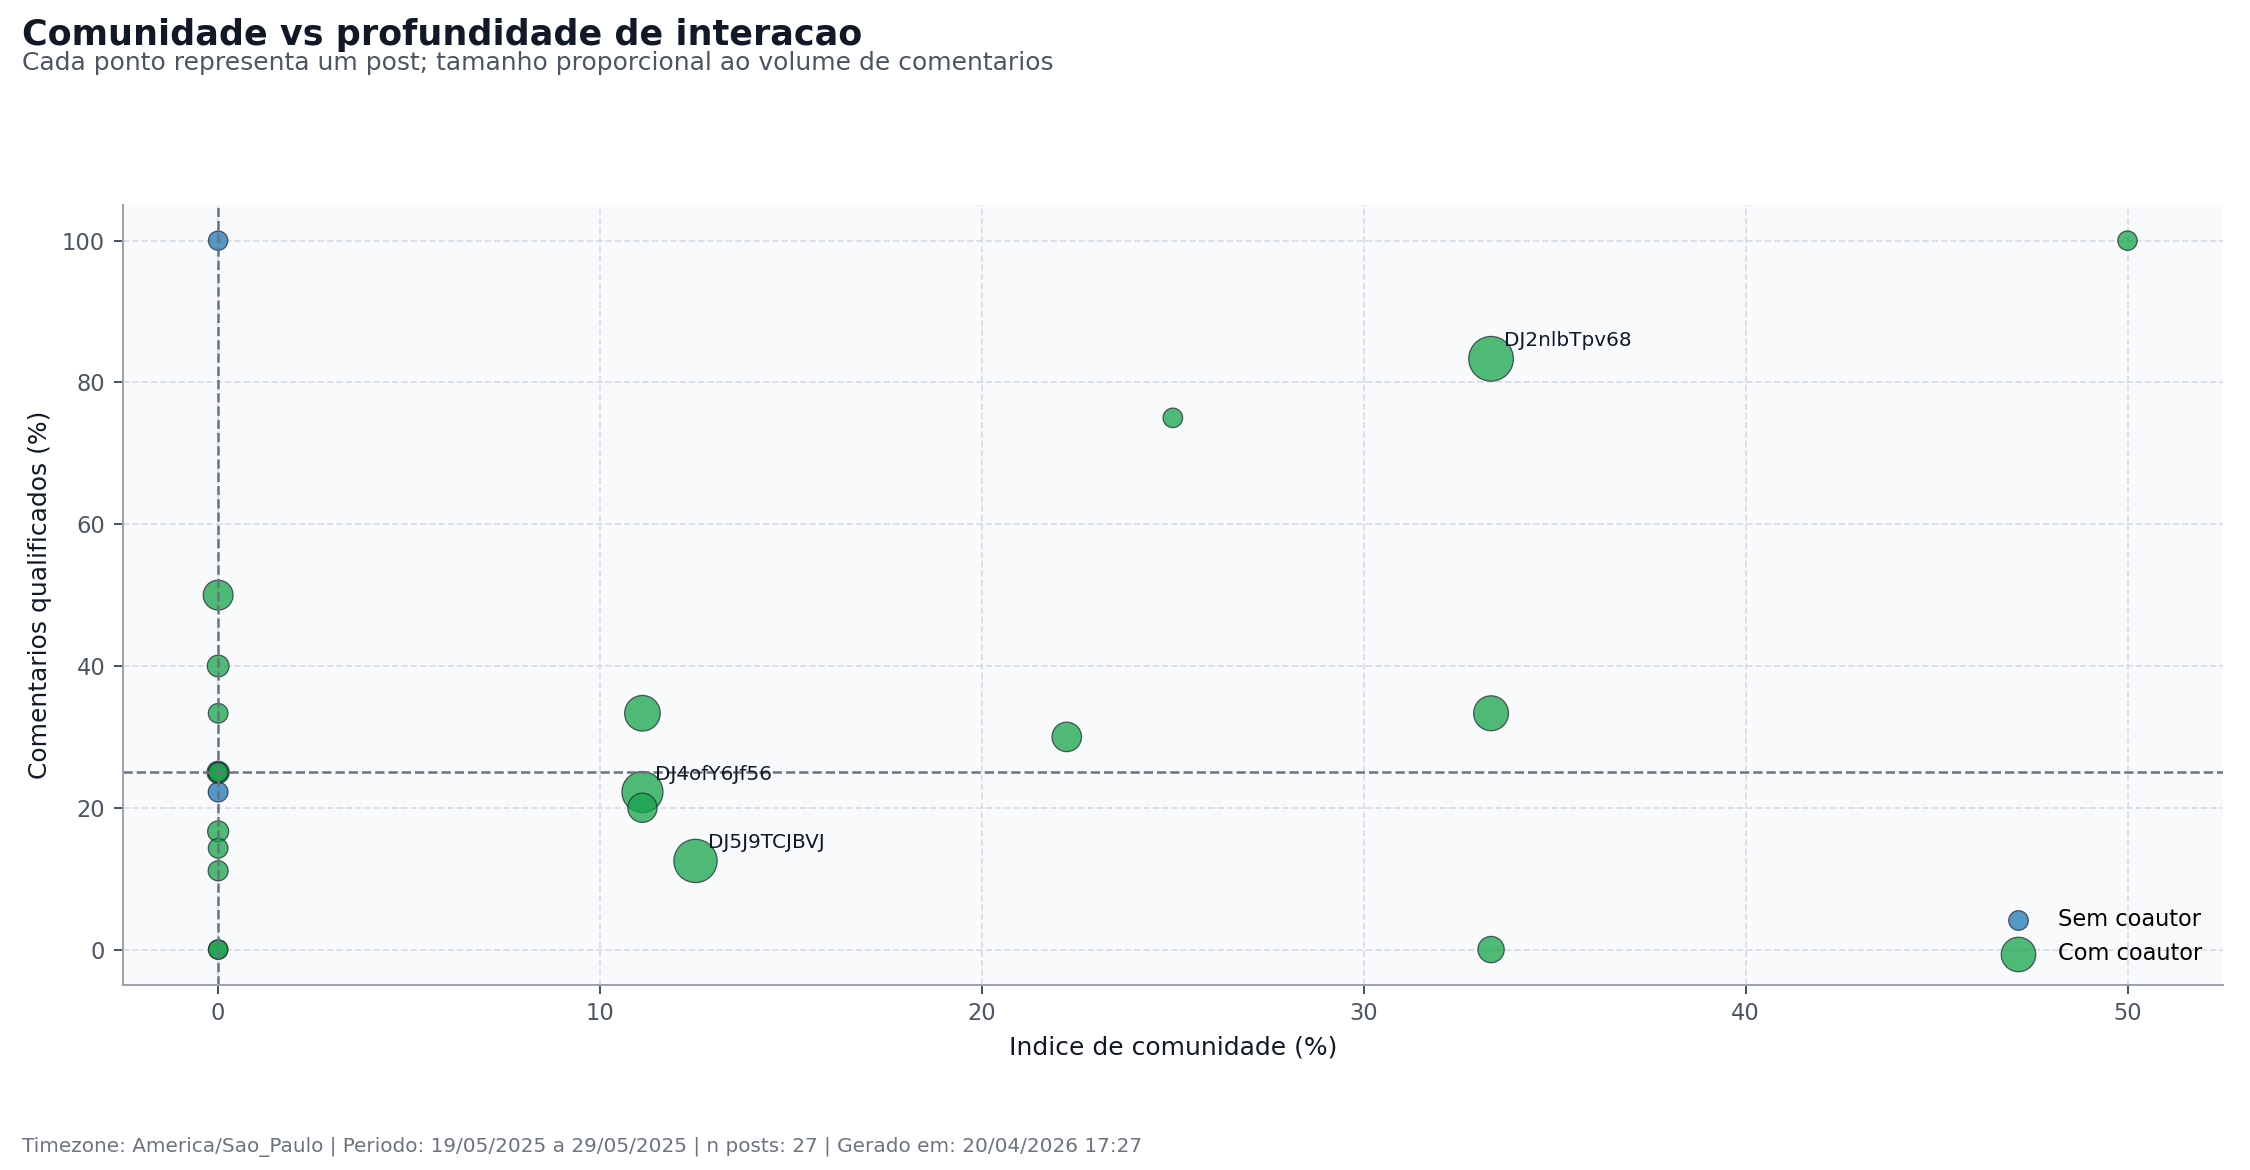
\includegraphics[width=0.93\textwidth]{charts/community_vs_quality.png}
\caption{Figura 7: Comunidade vs profundidade de interacao}
\end{figure}
\textit{Leitura rapida: Relaciona profundidade da conversa e sinal de comunidade.}

\section{Riscos e limites em linguagem simples}
\begin{itemize}
\item Quatro shortcodes nao tinham planilha de comentarios no recorte; isso reduz comparabilidade entre posts.
\item Em parte dos posts, visualizacoes nao estavam disponiveis; por isso algumas metricas por view aparecem como n/d.
\item latestComments e uma amostra recente de comentarios, nao o historico completo de cada publicacao.
\item Dados de seguidores, relacao seguidor/seguindo e perfil privado/publico da audiencia nao estao completos na fonte.
\item Lifts e correlacoes mostram associacao e ajudam a priorizar testes, mas nao comprovam causalidade sozinhos.
\end{itemize}
\section{Anexo tecnico essencial}
\subsection{Cobertura de arquivos por shortcode}
\begin{table}[H]
\centering
\scriptsize
\begin{adjustbox}{max width=\textwidth}
\begin{tabular}{l r r r}
\toprule
shortcode & has post & has comments & has owners \\
\midrule
DJ1\_MTEuA-i & 1 & 0 & 0 \\
DJ1oIOktsNX & 1 & 0 & 0 \\
DJ2nlbTpv68 & 1 & 1 & 1 \\
DJ48NUpJ544 & 1 & 1 & 1 \\
DJ4ofY6Jf56 & 1 & 1 & 1 \\
DJ4xlSdy-3m & 1 & 1 & 1 \\
DJ5AkVwJLXy & 1 & 1 & 1 \\
DJ5J9TCJBVJ & 1 & 1 & 1 \\
DJ630KnRcyp & 1 & 1 & 1 \\
DJ6unk6RCfx & 1 & 1 & 1 \\
DJ7jekBJKgG & 1 & 1 & 1 \\
DJ7XmcexhRk & 1 & 1 & 1 \\
DJ7ZoL4J2l- & 1 & 1 & 1 \\
DJ90M-cvd\_9 & 1 & 1 & 1 \\
DJ9bfPfRMcs & 1 & 1 & 1 \\
DJ9NCJqOH35 & 1 & 1 & 1 \\
DJ9ROIsNQhe & 1 & 0 & 0 \\
DKAHqt4x3uU & 1 & 1 & 1 \\
DKAkG0EpeK7 & 1 & 1 & 1 \\
DKH12WeAaO7 & 1 & 1 & 1 \\
DKHqNAsiCOw & 1 & 1 & 1 \\
DKHvDV\_NcFc & 1 & 0 & 0 \\
DKIPG0Hp-MT & 1 & 1 & 1 \\
DKK1ISuO5qS & 1 & 1 & 1 \\
DKPaci-t7V9 & 1 & 1 & 1 \\
DKPeLWNtI9U & 1 & 1 & 1 \\
DKQG98CJb9r & 1 & 1 & 1 \\
\bottomrule
\end{tabular}
\end{adjustbox}
\caption{Cobertura de arquivos por shortcode}
\label{tab:estrutura}
\end{table}

\subsection{Resumo de owners}
\begin{table}[H]
\centering
\scriptsize
\begin{adjustbox}{max width=\textwidth}
\begin{tabular}{r r r r r}
\toprule
total owner rows & owners unicos & percent verified & dados followers disponiveis & dados privacidade disponiveis \\
\midrule
136 & 129 & 2.21\% & 0 & 0 \\
\bottomrule
\end{tabular}
\end{adjustbox}
\caption{Resumo de owners}
\label{tab:owners}
\end{table}

\subsection{Proxy de video (duracao x retencao)}
\begin{table}[H]
\centering
\scriptsize
\begin{adjustbox}{max width=\textwidth}
\begin{tabular}{r r r r r}
\toprule
video posts & corr duracao visualizacoes & corr duracao comments per view & media duracao & mediana duracao \\
\midrule
13 & -0.6131 & 0.2302 & 120.12 & 92.72 \\
\bottomrule
\end{tabular}
\end{adjustbox}
\caption{Proxy de video (duracao x retencao)}
\label{tab:video}
\end{table}

\subsection{Topicos de legenda}
\begin{table}[H]
\centering
\scriptsize
\begin{adjustbox}{max width=\textwidth}
\begin{tabular}{l l l l}
\toprule
source & topic id & terms & metodo \\
\midrule
legenda & topico\_1 & 2025, vagas, internacional, santa, maria, rural & lda\_sklearn \\
legenda & topico\_2 & sobre, site, dia, link, bio, confira & lda\_sklearn \\
legenda & topico\_3 & silveira, zeloufsm, silveirapodrao, campus, pro, caninos & lda\_sklearn \\
legenda & topico\_4 & extensao, comunidade, cultura, campus, reitoria, 18h & lda\_sklearn \\
\bottomrule
\end{tabular}
\end{adjustbox}
\caption{Topicos de legenda}
\label{tab:topics\_legenda}
\end{table}

\subsection{Topicos de comentarios}
\begin{table}[H]
\centering
\scriptsize
\begin{adjustbox}{max width=\textwidth}
\begin{tabular}{l l l l}
\toprule
source & topic id & terms & metodo \\
\midrule
comentarios & topico\_1 & parabens, maria, santa, pena, sabe, resultado & lda\_sklearn \\
comentarios & topico\_2 & ufsm, gente, extensao, agenda, historia, deixa & lda\_sklearn \\
comentarios & topico\_3 & silveira, muito, desde, quando, hoje, bom & lda\_sklearn \\
comentarios & topico\_4 & projeto, todos, cara, animais, deus, amo & lda\_sklearn \\
\bottomrule
\end{tabular}
\end{adjustbox}
\caption{Topicos de comentarios}
\label{tab:topics\_comments}
\end{table}

\section{Conclusao}
Com os dados disponiveis, a estrategia recomendada e testar formato, horario e coautoria em ciclos curtos, acompanhando comentarios qualificados e sinais de comunidade para ajustar pauta e distribuicao.
\end{document}
